\documentclass[10pt,a4paper]{ULBreport}
\usepackage[utf8]{inputenc}
\sceau{pic/official_logos/sceauULB.png}
\graphicspath{ {./pic/} }
\usepackage{multirow}
\usepackage{listings}
\usepackage{color} 
\usepackage{setspace} 
\usepackage{amsmath}
\usepackage{hyperref}
\usepackage{pdfpages}
\usepackage{biblatex}
\usepackage{floatrow}
\usepackage{subcaption} 
\usepackage{siunitx}
\usepackage[many]{tcolorbox}
\usepackage{multirow}
\usepackage{listings}
\usepackage[dvipsnames]{xcolor}
\usepackage{fancyvrb}

\usepackage{xstring}
\usepackage{etoolbox}

% Colors



\begin{document} 


	\titleULB{
	title={CmOS},
    studies={MA1-IRELE},
    course ={OS and security},
    author={\textit{Author :} \\ Emmeran Colot },
    date={\textbf{Academic year :} \\ 2024 - 2025},
    teacher={\textit{Professor : } \\ Prof. B. Da Silva},
    logo={pic/official_logos/logos.jpg},
    manyAuthor
	}

%\listoftables % ToC for tables

%\listoffigures % ToC for figures

\chapter{Introduction}

In this report, a comparison of two ways of storing files is made. There is a main focus on how those storage systems work, followed by a comparison of their performance. \\

The project was initially named \textit{CmOS} for \textit{C modeled OS} as it was supposed to implement more than only a storage system. The whole code is available on github\footnote{\href{https://github.com/e-colot/CmOS}{https://github.com/e-colot/CmOS}} and one can see that the basic building blocks for a complete OS are present. It includes registers definition, a custom ISA, a compiler and an interpreter for going from assembly to binary and then execute it and so on, but they will not be discussed as the project objective has changed to the study of storage systems. It is a smaller topic but there is still a lot to say about it. 

Finally, there are a few remarks:
\begin{itemize}
    \item This whole project has been built by hand with no external source. This means that the two systems are not based on any existing system but only on the knowledge acquired during the course and on some personal ideas.
    \item In the following, the terms \textit{file system} and \textit{storage system} will be used interchangeably
    \item Except when specifically mentioned, the term \textit{disk} will refer to the simulated disk.
\end{itemize}






\chapter{Background}

As everything is built from scratch, there is not a lot of prerequisite knowledge needed to understand this report. However, a few concepts are important to understand how the two systems work.

\section{disk}
\label{sec:disk}

The disk is where files are stored on a computer and it can be seen as a big vector of bytes. To read or write some data, an address is given and the driver will read or write the data at that address. A real disk will often have different sectors with a longer access time when changing sectors. \\

In the simulation, the disk is a file on the computer of which the size is fixed by a parameter. Because of this, there is no access time when changing sectors. However, because of paging (which will be explained later) and depending on the computer on which the simulation is run, the access time could indeed be longer when reading or writing data at addresses that are far away from each other but this is, once again, outside of the scope of this analysis. \\

\section{Paging}
\label{sec:paging}

When storing data in memory, it would be inefficient to have data blocks of varying sizes. This is why the memory is divided into blocks of fixed size. Each of those blocks is called a \textit{page} and the size of a page is called the \textbf{page size}. This size will be an important parameter in the following.

\section{File system}
\label{sec:filesystem}

The file system is in charge of managing the data on the disk. It is responsible for writing files, accessing written files and deleting them. It might have additional features but those are sufficient for a working file system and the one built here only implement those basic operations.







\chapter{Description of the storage systems}

\section{generalities}
\subsection{Variable page size}
As described in section \ref{sec:paging}, both file systems will use paging to store data. The page size is variable and can be set when creating the file system. Building a variable page size system is not a difficult task unless it aims to be efficient. Both of the systems built here have been designed to be efficient so this single feature has doubled the development time.
\subsection{Folders}
For the sake of simplicity, the two systems will not implement folders. This is a choice that is often made for small size operating systems such as for RTOS\footnote{Real Time Operating System}.
\subsection{Addressing bytes}
The disk is split into pages of a fixed size but when trying to write or read a page, there must be a way of pointing to it. Because the disk size and the page size are parameters, one can not assume a single byte address will be enough to address all the pages. \\
A disk of 256 kB with a page size of 256 bytes will have 1024 pages and a single byte address can only go up to 255. This means that a single byte address will not be enough to address all the pages. This is why the number of bytes used to address a page, referred to as \textbf{addressing bytes} or $A_b$, is variable and is computed as follows:
\begin{equation*}
    A_b = \lceil \log_2\left(\frac{\text{disk size}}{\text{page size}}\right) \rceil
\end{equation*}
The complexity of addressing with a variable number of bytes is that, depending on the dimensions of the disk and the page size, the place needed to store an address can vary, making the disk content vary. As the disk is only a file on the computer running the simulation, it is limited in size so more than 4 addressing bytes are not implemented. This would correspond to a disk of 64 GB with a page size of 16 bytes\footnote{This value of 16 bytes is not chosen randomly, it will be explained later.}.
\subsection{File allocation table}
Somewhere on the disk, there is a space reserved for the file allocation table (FAT). This table is used to store the information about the files on the disk. All the information related to a file will be referred to as an \textit{entry} or a \textit{file entry}.\\
It stores at least the following information:
\begin{itemize}
    \item A way to uniquely identify the file
    \item The address of the first page of the file
\end{itemize}
and it can store more information, as will be shown later in one of the systems.
\subsection{File identifier}
The file identifier is, as described in the previous section, a way to uniquely identify a file. It is generally a string of characters, corresponding to the name of the file. Because this simulation aims to be efficient and it can work with a really small disk (most of the tests were done with a 4kB disk), having a string would quickly fill the disk. \\
For this reason, the file identifier is simply a number. This number is different of zero, which is a reserved number for an empty file. To make sure that every file is can have a unique identifier, this \textbf{ID} is stored on the same number of bytes as the addressing bytes. As each file is stored on at least one page, which address holds on $A_b$ bytes, using the same number of bytes for the ID will be enough to store the ID of the file. \\
When adding a file, the given ID is checked against the IDs found in the FAT to avoid duplicates and an error mechanism is implemented to handle this case. 
\subsection{File terminator}
Because the files are stored in pages, there often are bytes at the end that are not data. Because only the number of pages used to store the data is known (and not the number of bytes), there is a need to differentiate the bytes that compose the data and the ones that are not and this is the interest of having a file terminator. \\
At the end of the file, \texttt{0x00} is added and this is the file terminator symbol. It is then followed by a padding: the rest of the page is filled with \texttt{0xFF}. If this padding was not made, there could be a risk of having another \texttt{0x00} that would be interpreted as the terminator.

\section{Linked list allocation system}
\label{sec:linkedlist}
\subsection{Description}
The first system is a linked list allocation system. This means that the pages of a file are not stored next to each other on the disk. Instead, each page contains at its beginning a pointer to the next page of the file. The last page has a pointer to zero, indicating that it is the last page of the file.
\subsection{Bitmap}
Because the pages are not stored next to each other, there is a need for a way to know which pages are free to be used and which ones are already used. It is for this reason that a bitmap is present at the beginning of the disk. \\
Each bit of the bitmap corresponds to a page on the disk and is set to 1 if the page is used and to 0 if it is free.
\subsection{FAT structure}
The first FAT page is always placed right after the bitmap. As more files are added, the FAT will grow and at some point, a single page will not be enough. The next page is then chosen among the free pages (found in the bitmap) and the previous page will point to the new page. This allows the FAT to grow as needed and make this system scalable. 
\begin{figure}[H]
    \floatbox[{\capbeside\thisfloatsetup{capbesideposition={right,top},capbesidewidth=0.5\textwidth}}]{figure}[\FBwidth]
    {\caption{The structure of the File Allocation Table (FAT) in the linked list allocation system.\\ It starts with $2 A_b$ bytes linking to the previous and the next FAT pages. It is then followed by \textit{entries} of $2 A_b$ each with the ID of the file and the address of the first page where the file is written.\\ Because each little box on the figure contains $A_b$ bytes and because $A_b$ is not bigger than 4, a page size smaller than 16 could lead to issues. In the case of a page size of 15 and $A_b = 4$ (with a huge disk size for instance), the first row will already use 8 out of the 15 bytes. There will then not be enough bytes left to write a single file entry in the page, making it useless}\label{fig:FAT_LL}}
    {\includegraphics[width=0.4\textwidth]{FAT_LL.png}}
\end{figure}
\subsection{Finding a free page}
For writing operations, there is often the need to find a page that is not used. Because the files must not be stored one after the other, the address returned is purely random, but it still must be an unused one. The first approach that was implemented was a \textit{Random Access} method:
\begin{enumerate}
    \item Take a random address < number of pages
    \item If it is already used, go back to \textbf{1.}
    \item If not, return the address
\end{enumerate}
It has been replaced later on by the \textit{Continue Until Found} method:
\begin{enumerate}
    \item Take a random address < number of pages
    \item If it is already used, check the next address and go to \textbf{2.}
    \item If not, return the address
\end{enumerate}
To compare the two approaches for finding a free page, a simulation was run where the disk was gradually filled, and the time taken to find a free page was recorded. The results are shown in Figure \ref{fig:findFreePageTime}. \\
\begin{figure}
    \centering
    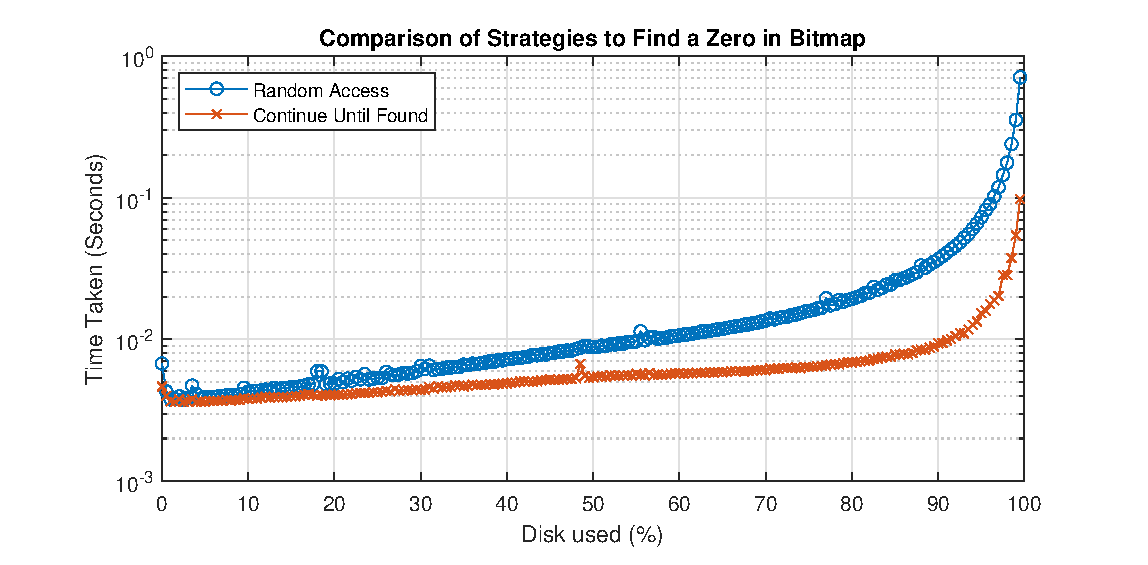
\includegraphics[width=1\textwidth]{findFreePage.eps}
    \caption{Comparison of the time taken to find a free page as the disk fills up. This simulation was done with a toy script in Matlab, not the real system}
    \label{fig:findFreePageTime}
\end{figure}
The second approach, which checks the next address sequentially, performs significantly better when the disk is nearly full, which was expected as it has the certitude of finding a free page after having searched through the whole bitmap.
\subsection{Adding a file}
A simplified version of the algorithm to add a file is shown on the logical diagram \ref{fig:Logic_add_LL}. There are a lot of checks to be done when adding a file and those are not included in the diagram. \\
For instance, if no page new page is found for writing after the file entry has been put in the FAT (inside the while loop in \ref{fig:Logic_add_LL}), it means that the disk is full. However, as the file is not entirely written, it cannot stay there as it could potentially be read and it would not be the same data as what was given. The fix for it is to mark the last page as the end of the file with a pointer to 0 (see the next section to understand why it is important) and then remove the file.
\begin{figure}
    \centering
    \includegraphics[width=0.8\textwidth]{Logic_add_LL.png}
    \caption{Logical diagram of the algorithm to add a file in the linked list allocation system}
    \label{fig:Logic_add_LL}
\end{figure}
\subsection{Removing a file}
To remove a file, its entry must be removed from the FAT and all the pages used to store the file must be cleared in the bitmap. Removing the entry is straightforward: it cycles through the FAT pages and search for the ID. When found, it sets the ID to 0 to indicate that there is no more file\footnote{This is the reason why the ID 0 cannot be used by any file} and the address of the first page is stored. From there, it sets the current page as free in the bitmap and load the next page of the file (using the pointer at the start of the current page) until the next address is 0, which indicates the end of the file.
\subsection{Loading a file}
There is not much to say about this. It proceeds like for a page removal except that instead of marking the page free in the bitmap, it gets rid of the pointer to the next page and load the data in a buffer to be sent back.
\subsection{FAT reorganization}
Once in 10 times a file is removed, a FAT reorganization takes place. It will fill the holes in the first FAT pages (entries with ID = 0) with entries that are in the last pages of the FAT. This allows to empty the last FAT pages and to remove them. It frees some pages which can then be used to store more files.

\section{Contiguous allocation system}









\chapter{Experimental results}







\chapter{Conclusion}

%\printglossary

%\printglossary[type=\acronymtype]

%Bibliography
%\nocite{*}
%\printbibliography[type=article,title=Articles]

\end{document}	